
\tikzset{every picture/.style={line width=0.75pt}} %set default line width to 0.75pt        

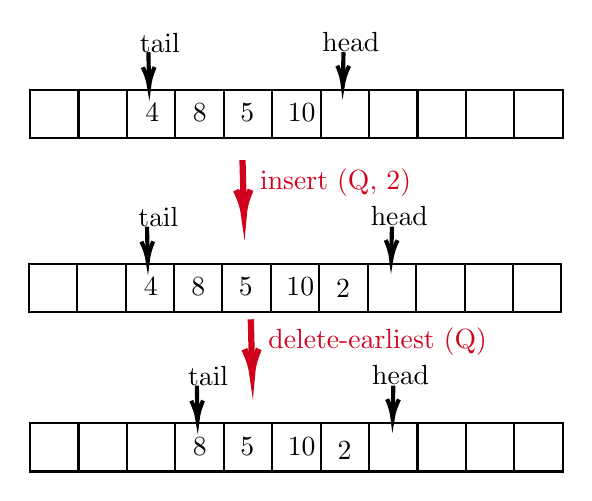
\begin{tikzpicture}[x=0.5pt,y=0.5pt,yscale=-1,xscale=1]
%uncomment if require: \path (0,337); %set diagram left start at 0, and has height of 337

%Shape: Grid [id:dp4942254527972789] 
\draw  [draw opacity=0] (11,49) -- (396,49) -- (396,84) -- (11,84) -- cycle ; \draw   (46,49) -- (46,84)(81,49) -- (81,84)(116,49) -- (116,84)(151,49) -- (151,84)(186,49) -- (186,84)(221,49) -- (221,84)(256,49) -- (256,84)(291,49) -- (291,84)(326,49) -- (326,84)(361,49) -- (361,84) ; \draw    ; \draw   (11,49) -- (396,49) -- (396,84) -- (11,84) -- cycle ;
%Straight Lines [id:da011203202476256058] 
\draw [line width=1.5]    (96.5,22) -- (96.94,44) ;
\draw [shift={(97,47)}, rotate = 268.85] [color={rgb, 255:red, 0; green, 0; blue, 0 }  ][line width=1.5]    (14.21,-4.28) .. controls (9.04,-1.82) and (4.3,-0.39) .. (0,0) .. controls (4.3,0.39) and (9.04,1.82) .. (14.21,4.28)   ;
%Straight Lines [id:da9859159949652865] 
\draw [line width=1.5]    (237.5,22) -- (237.06,43) ;
\draw [shift={(237,46)}, rotate = 271.19] [color={rgb, 255:red, 0; green, 0; blue, 0 }  ][line width=1.5]    (14.21,-4.28) .. controls (9.04,-1.82) and (4.3,-0.39) .. (0,0) .. controls (4.3,0.39) and (9.04,1.82) .. (14.21,4.28)   ;
%Shape: Grid [id:dp8078577975258915] 
\draw  [draw opacity=0] (10,175) -- (395,175) -- (395,210) -- (10,210) -- cycle ; \draw   (45,175) -- (45,210)(80,175) -- (80,210)(115,175) -- (115,210)(150,175) -- (150,210)(185,175) -- (185,210)(220,175) -- (220,210)(255,175) -- (255,210)(290,175) -- (290,210)(325,175) -- (325,210)(360,175) -- (360,210) ; \draw    ; \draw   (10,175) -- (395,175) -- (395,210) -- (10,210) -- cycle ;
%Straight Lines [id:da10073653551255601] 
\draw [line width=1.5]    (95.5,148) -- (95.94,170) ;
\draw [shift={(96,173)}, rotate = 268.85] [color={rgb, 255:red, 0; green, 0; blue, 0 }  ][line width=1.5]    (14.21,-4.28) .. controls (9.04,-1.82) and (4.3,-0.39) .. (0,0) .. controls (4.3,0.39) and (9.04,1.82) .. (14.21,4.28)   ;
%Straight Lines [id:da38679209155686467] 
\draw [line width=1.5]    (272.5,148) -- (272.06,169) ;
\draw [shift={(272,172)}, rotate = 271.19] [color={rgb, 255:red, 0; green, 0; blue, 0 }  ][line width=1.5]    (14.21,-4.28) .. controls (9.04,-1.82) and (4.3,-0.39) .. (0,0) .. controls (4.3,0.39) and (9.04,1.82) .. (14.21,4.28)   ;
%Shape: Grid [id:dp8559849663357562] 
\draw  [draw opacity=0] (11,290) -- (396,290) -- (396,325) -- (11,325) -- cycle ; \draw   (46,290) -- (46,325)(81,290) -- (81,325)(116,290) -- (116,325)(151,290) -- (151,325)(186,290) -- (186,325)(221,290) -- (221,325)(256,290) -- (256,325)(291,290) -- (291,325)(326,290) -- (326,325)(361,290) -- (361,325) ; \draw    ; \draw   (11,290) -- (396,290) -- (396,325) -- (11,325) -- cycle ;
%Straight Lines [id:da6868992534526999] 
\draw [line width=1.5]    (131.5,263) -- (131.94,285) ;
\draw [shift={(132,288)}, rotate = 268.85] [color={rgb, 255:red, 0; green, 0; blue, 0 }  ][line width=1.5]    (14.21,-4.28) .. controls (9.04,-1.82) and (4.3,-0.39) .. (0,0) .. controls (4.3,0.39) and (9.04,1.82) .. (14.21,4.28)   ;
%Straight Lines [id:da16952414255259152] 
\draw [line width=1.5]    (273.5,263) -- (273.06,284) ;
\draw [shift={(273,287)}, rotate = 271.19] [color={rgb, 255:red, 0; green, 0; blue, 0 }  ][line width=1.5]    (14.21,-4.28) .. controls (9.04,-1.82) and (4.3,-0.39) .. (0,0) .. controls (4.3,0.39) and (9.04,1.82) .. (14.21,4.28)   ;
%Straight Lines [id:da21618036120919215] 
\draw [color={rgb, 255:red, 208; green, 2; blue, 27 }  ,draw opacity=1 ][line width=2.25]    (164.5,100) -- (165.4,135) ;
\draw [shift={(165.5,139)}, rotate = 268.53] [color={rgb, 255:red, 208; green, 2; blue, 27 }  ,draw opacity=1 ][line width=2.25]    (17.49,-5.26) .. controls (11.12,-2.23) and (5.29,-0.48) .. (0,0) .. controls (5.29,0.48) and (11.12,2.23) .. (17.49,5.26)   ;
%Straight Lines [id:da7278943927425445] 
\draw [color={rgb, 255:red, 208; green, 2; blue, 27 }  ,draw opacity=1 ][line width=2.25]    (170.5,215) -- (171.4,250) ;
\draw [shift={(171.5,254)}, rotate = 268.53] [color={rgb, 255:red, 208; green, 2; blue, 27 }  ,draw opacity=1 ][line width=2.25]    (17.49,-5.26) .. controls (11.12,-2.23) and (5.29,-0.48) .. (0,0) .. controls (5.29,0.48) and (11.12,2.23) .. (17.49,5.26)   ;

% Text Node
\draw (88,6) node [anchor=north west][inner sep=0.75pt]   [align=left] {tail};
% Text Node
\draw (220,5) node [anchor=north west][inner sep=0.75pt]   [align=left] {head};
% Text Node
\draw (92,57) node [anchor=north west][inner sep=0.75pt]   [align=left] {$\displaystyle 4$};
% Text Node
\draw (126.33,57) node [anchor=north west][inner sep=0.75pt]   [align=left] {$\displaystyle 8$};
% Text Node
\draw (160.66,57) node [anchor=north west][inner sep=0.75pt]   [align=left] {$\displaystyle 5$};
% Text Node
\draw (195,57) node [anchor=north west][inner sep=0.75pt]   [align=left] {$\displaystyle 10$};
% Text Node
\draw (87,132) node [anchor=north west][inner sep=0.75pt]   [align=left] {tail};
% Text Node
\draw (255,131) node [anchor=north west][inner sep=0.75pt]   [align=left] {head};
% Text Node
\draw (91,183) node [anchor=north west][inner sep=0.75pt]   [align=left] {$\displaystyle 4$};
% Text Node
\draw (125.33,183) node [anchor=north west][inner sep=0.75pt]   [align=left] {$\displaystyle 8$};
% Text Node
\draw (159.66,183) node [anchor=north west][inner sep=0.75pt]   [align=left] {$\displaystyle 5$};
% Text Node
\draw (194,183) node [anchor=north west][inner sep=0.75pt]   [align=left] {$\displaystyle 10$};
% Text Node
\draw (123,247) node [anchor=north west][inner sep=0.75pt]   [align=left] {tail};
% Text Node
\draw (256,246) node [anchor=north west][inner sep=0.75pt]   [align=left] {head};
% Text Node
\draw (126.33,298) node [anchor=north west][inner sep=0.75pt]   [align=left] {$\displaystyle 8$};
% Text Node
\draw (160.66,298) node [anchor=north west][inner sep=0.75pt]   [align=left] {$\displaystyle 5$};
% Text Node
\draw (195,298) node [anchor=north west][inner sep=0.75pt]   [align=left] {$\displaystyle 10$};
% Text Node
\draw (175,104) node [anchor=north west][inner sep=0.75pt]   [align=left] {\textcolor[rgb]{0.82,0.01,0.11}{insert (Q, 2)}};
% Text Node
\draw (230,184) node [anchor=north west][inner sep=0.75pt]   [align=left] {$\displaystyle 2$};
% Text Node
\draw (181,219) node [anchor=north west][inner sep=0.75pt]   [align=left] {\textcolor[rgb]{0.82,0.01,0.11}{delete-earliest (Q)}};
% Text Node
\draw (231,301) node [anchor=north west][inner sep=0.75pt]   [align=left] {$\displaystyle 2$};


\end{tikzpicture}

